\documentclass[12pt,a4paper]{article}

% Paquetes básicos
\usepackage[utf8]{inputenc}
\usepackage[T1]{fontenc}
\usepackage[spanish]{babel}
\usepackage{amsmath, amssymb}
\usepackage{siunitx} % Ángulos
\usepackage{graphicx}
\usepackage{float}
\usepackage{geometry}
\geometry{margin=2.5cm}
\usepackage{hyperref}
\usepackage{caption}
\usepackage{subcaption}
\usepackage{setspace}
\usepackage{multirow}
\usepackage{minted}  % Códigos
\usepackage{gensymb} % Grados: "°"
\graphicspath{{Figuras/}}
\onehalfspacing


% Datos
\author{Nombre y Apellido \\ Legajo: XXXXX}
\date{\today}

\begin{document}

% Carátula personalizada
\begin{titlepage}
    \centering
    \includegraphics[width=0.25\textwidth]{escudo.png} 
    \hspace{1cm}
    \includegraphics[width=0.3\textwidth]{download.png} \\[1cm]

    {\large \textbf{UNIVERSIDAD NACIONAL DE CÓRDOBA} \\[0.5cm]}
    {\large \textbf {FACULTAD DE CIENCIAS EXACTAS, FÍSICAS Y NATURALES} \\[1cm]}
    {\Large ANTENAS Y PROPAGACIÓN DE ONDAS\\[1cm]}

    \rule{\textwidth}{0.5pt} \\[0.5cm]
    {\Large \textbf{Trabajo Práctico N°1} \\[0.3cm]}
    {\Large \textbf{Diagramas de Radiación de la Antena Dipolo} \\[0.3cm]}
    \rule{\textwidth}{0.5pt} \\[1cm]

\begin{tabular}{l l}
\textbf{Profesor Titular:} & Ing. Jose Luis Amado. \\

\\
\textbf{Alumno:} Monja, Ernesto Joaquín. \\
\textbf{DNI:} 43.873.728 \\
\end{tabular}\\[3cm]

{\centering Año 2026 \par}

\end{titlepage}



% Índice
\tableofcontents
\newpage
\indent



\section{Introducción}
En el campo de las telecomunicaciones y el electromagnetismo, las antenas constituyen el eslabón fundamental que permite la transición de señales eléctricas guiadas a ondas electromagnéticas que se propagan en el espacio libre. Entre la vasta diversidad de geometrías existentes, la \textit{antena dipolo lineal} se destaca como la estructura radiante más elemental y exhaustivamente estudiada, sirviendo como bloque de construcción conceptual para sistemas y arreglos de antenas más complejos.

Una de las características principales para evaluar el desempeño, la cobertura y la directividad de cualquier antena es su \textit{diagrama de radiación}, una representación gráfica tridimensional (o cortes bidimensionales) que ilustra cómo se distribuye la energía radiada en las distintas direcciones del espacio. En el caso del dipolo, este patrón espacial no es estático ni genérico, sino que depende fuertemente de la longitud física del elemento $L$ en relación con la longitud de onda $\lambda$ de la señal de operación. Para caracterizar matemáticamente esta distribución espacial en la zona de campo lejano, se recurre al análisis del Factor de Forma $F(\theta)$. Esta función describe la dependencia angular de la intensidad del campo eléctrico radiado.

El presente trabajo práctico tiene como objetivo principal el estudio y la visualización teórica de los diagramas de radiación de la antena dipolo de longitud $L$. A partir de la aplicación analítica de las ecuaciones del Factor de Forma $F(\theta)$, se trazarán y analizarán los patrones de radiación resultantes para distintas relaciones de longitud, permitiendo comprender, de manera gráfica y matemática, cómo la geometría del elemento radiante define sus propiedades fundamentales de transmisión en el espacio.



\section{Desarrollo}
\subsection{Marco Teórico}
En la \autoref{fig:fig_1} se presenta un sistema de coordenadas cartesianas tridimensionales definido por los ejes $x$, $y$ y $z$:
\begin{figure}[H]
    \centering
    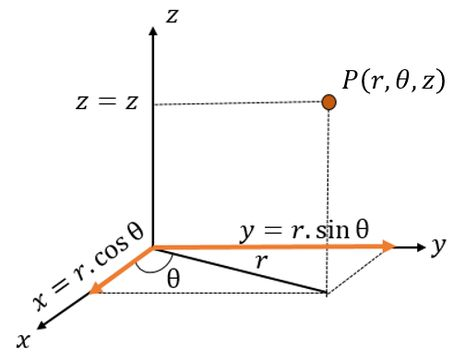
\includegraphics[width=0.5\linewidth]{Figura 1.png}
    \caption{Sistema de coordenadas cartesianas. [1]}
    \label{fig:fig_1}
\end{figure}

Si se coloca una antena dipolo de longitud $L$ en el centro de los ejes de referencia, se pueden desarrollar y obtener las expresiones para las magnitudes de los campos eléctricos y magnéticos en coordenadas esféricas según: [2]
\begin{equation}
    \begin{cases}
        \hat{E_{\theta}} = \frac{j \eta_{0} \hat{I}}{2 \pi r} e^{-j \beta_{0}r} \left[ \frac{\cos\left( \frac{\beta_{0}L}{2}\cos(\theta) \right) - \cos\left( \frac{\beta_{0}L}{2} \right)}{\sin(\theta)} \right] \ \left[\frac{V}{m}\right] \\[10pt]
        \hat{H_{\phi}} = \frac{j \hat{I}}{2\pi r} e^{-j \beta_{0}r} \left[ \frac{\cos\left( \frac{\beta_{0}L}{2}\cos(\theta) \right) - \cos\left( \frac{\beta_{0}L}{2} \right)}{\sin(\theta)} \right] \ \left[\frac{A}{m}\right]
    \end{cases}
    \label{eq_1}
\end{equation}

Nótese que en ambas ecuaciones de la \autoref{eq_1} existe un término común encerrado entre corchetes, el cual se denomina \textit{Factor de Forma} y se define como:
\begin{equation}
    \left| F(\theta) \right| = \left| \frac{\cos\left( \frac{\beta_{0}L}{2}\cos(\theta) \right) - \cos\left( \frac{\beta_{0}L}{2} \right)}{\sin(\theta)}\right|
    \label{eq_2}
\end{equation}

Al reemplazar $\beta_{0} = \frac{2\pi}{\lambda}$ en la \autoref{eq_2}, se llega a obtener una expresión del \textit{Factor de Forma} que depende de la longitud de onda tal que:
\begin{equation}
    \left| F(\theta) \right| = \left| \frac{\cos\left( \frac{\pi L}{\lambda}\cos(\theta) \right) - \cos\left( \frac{\pi L}{\lambda} \right)}{\sin(\theta)}\right|
    \label{eq_3}
\end{equation}

Como se ha mencionado en la introducción, las expresiones del Factor de Forma $F(\theta)$ son la base para trazar y definir los diagramas de radiación de una antena, los cuales se analizan en la sección siguiente.



\subsection{Simulación de los Diagramas de Radiación en Python}
Se propone diseñar un Script de Python [3] el cual permita definir a la función del Factor de Forma $F(\theta)$ según \autoref{eq_3}, donde le podamos pasar como parámetro la longitud de onda deseada y observamos como es el factor de forma que nos permitirá graficar como son los diagramas de radiación.

Se propone analizar los siguientes casos:
\begin{itemize}
    \item \underline{Diagrama de Radiación para $L = \frac{\lambda}{8}$:}
    \begin{figure}[H]
        \centering
        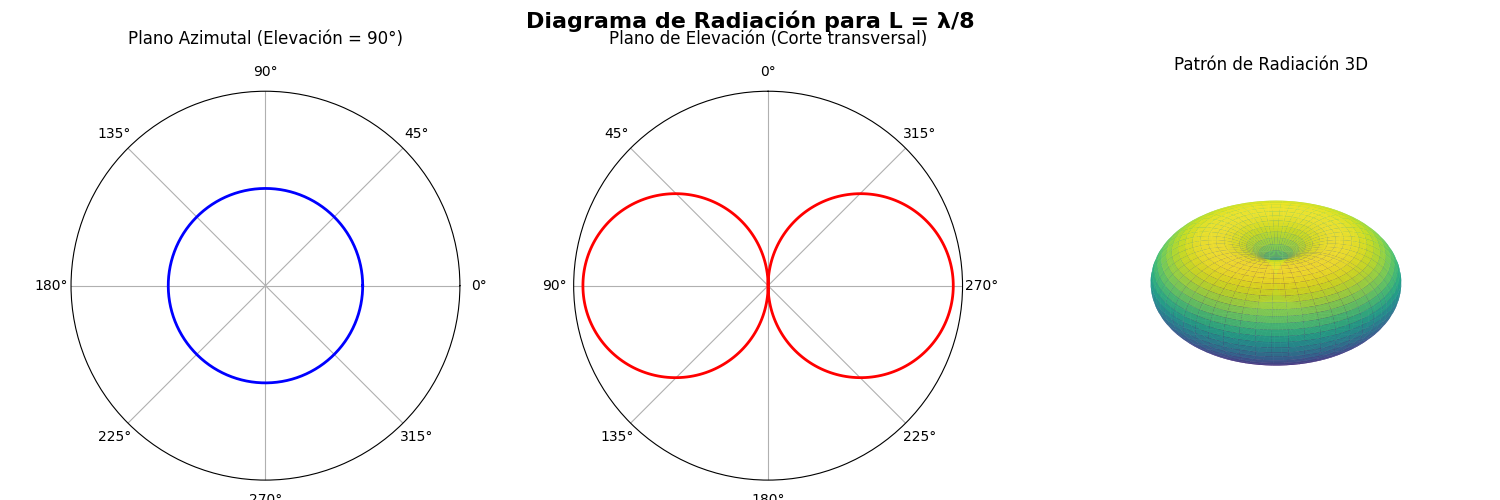
\includegraphics[width=1\linewidth]{Figura 2.png}
        \caption{Diagrama de Radiación para $L = \frac{\lambda}{8}$.}
        \label{fig:fig_2}
    \end{figure}
    
\item \underline{Diagrama de Radiación para $L = \frac{\lambda}{4}$:}
    \begin{figure}[H]
        \centering
        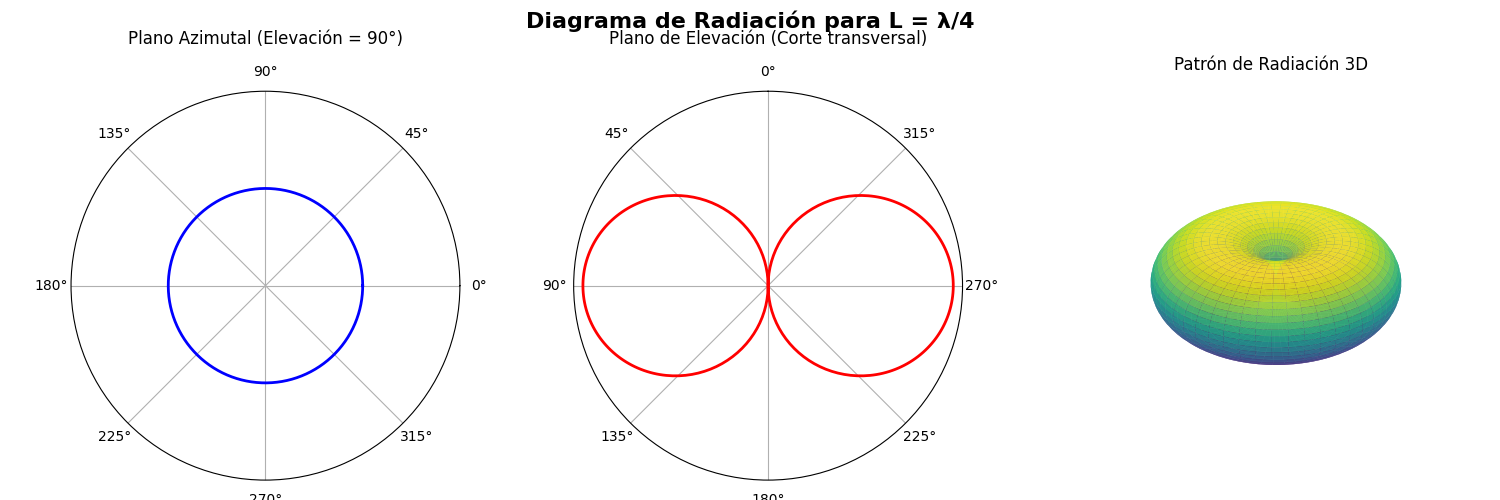
\includegraphics[width=1\linewidth]{Figura 3.png}
        \caption{Diagrama de Radiación para $L = \frac{\lambda}{4}$.}
        \label{fig:fig_3}
    \end{figure}

    \item \underline{Diagrama de Radiación para $L = \frac{\lambda}{2}$:}
    \begin{figure}[H]
        \centering
        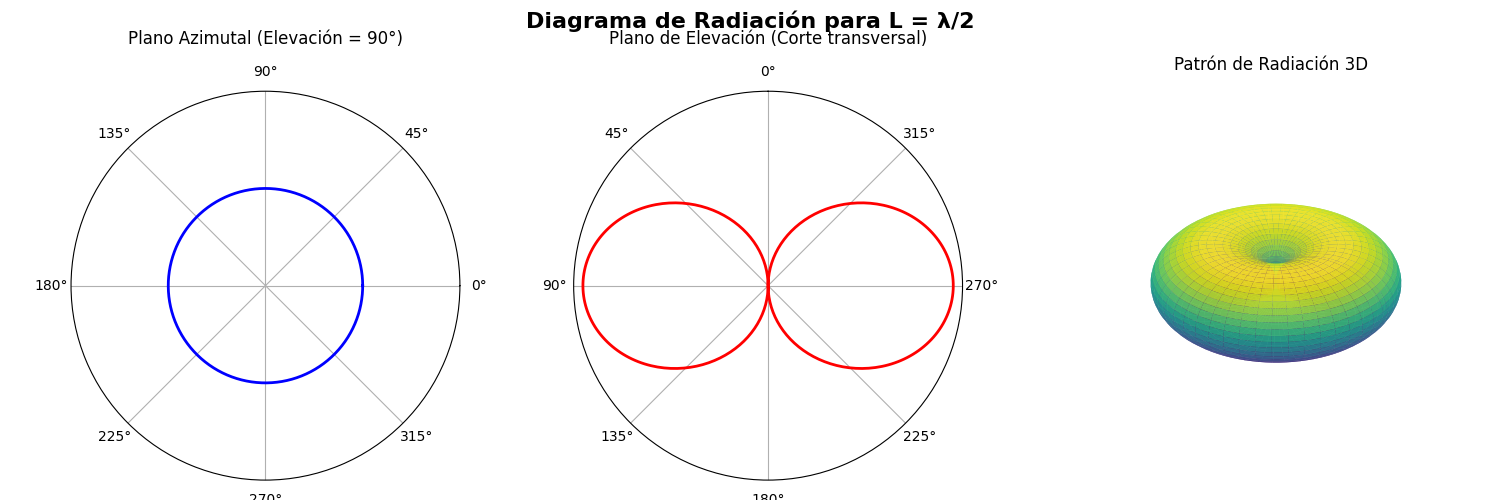
\includegraphics[width=1\linewidth]{Figura 4.png}
        \caption{Diagrama de Radiación para $L = \frac{\lambda}{2}$.}
        \label{fig:fig_4}
    \end{figure}

    \item \underline{Diagrama de Radiación para $L = \frac{3\lambda}{4}$:}
    \begin{figure}[H]
        \centering
        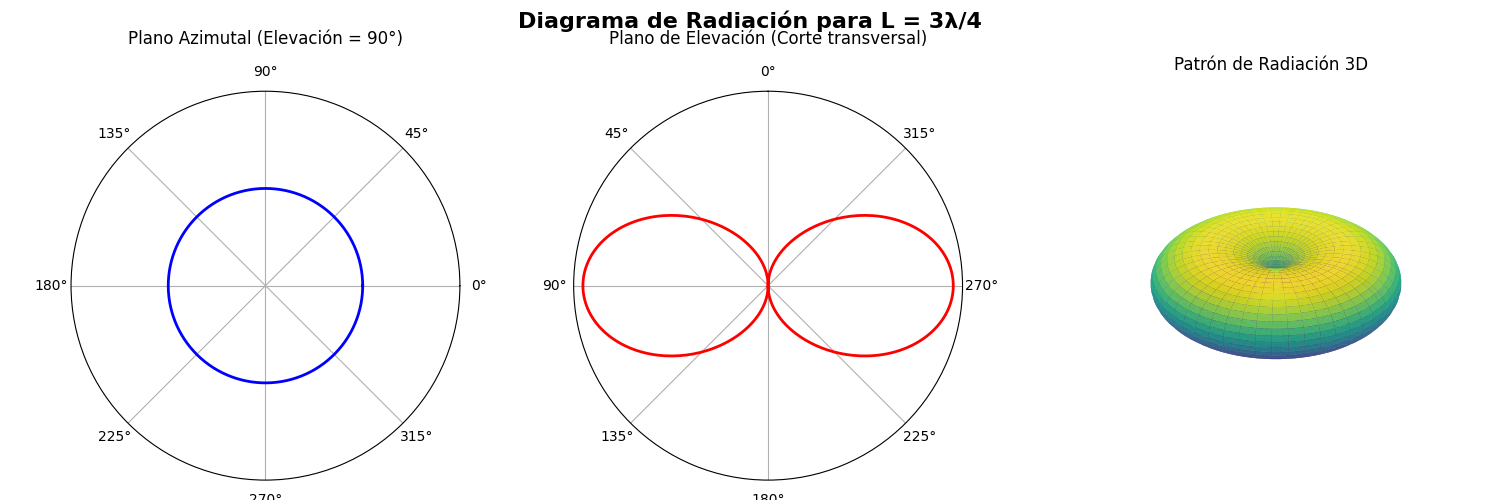
\includegraphics[width=1\linewidth]{Figura 5.png}
        \caption{Diagrama de Radiación para $L = \frac{3\lambda}{4}$.}
        \label{fig:fig_5}
    \end{figure}

    \item \underline{Diagrama de Radiación para $L = \lambda$:}
    \begin{figure}[H]
        \centering
        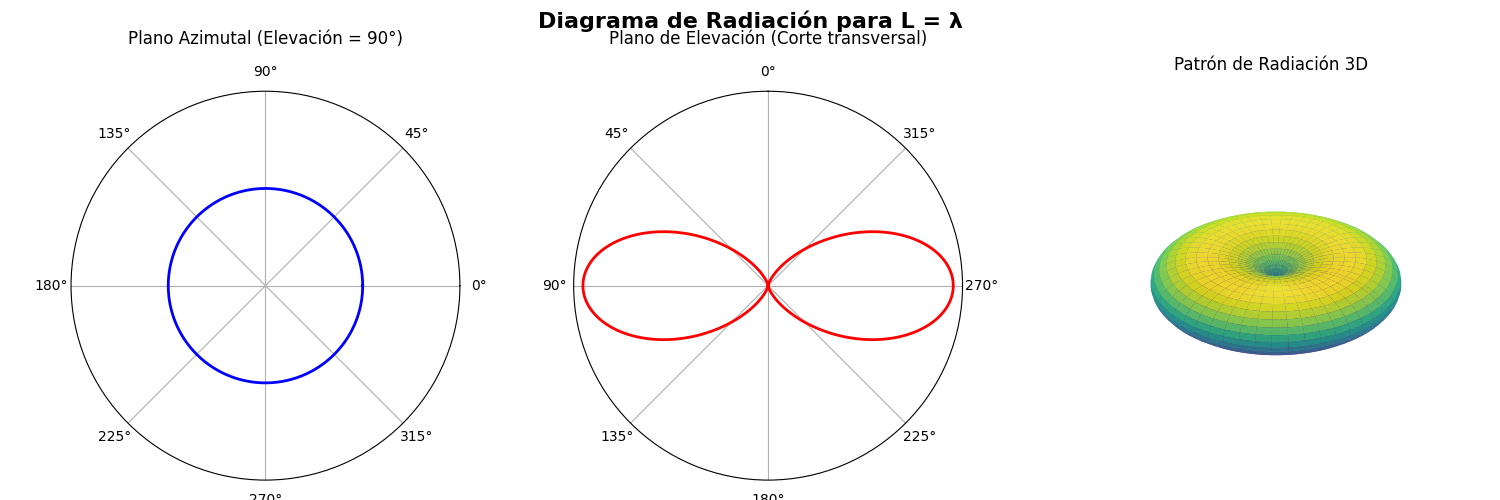
\includegraphics[width=1\linewidth]{Figura 6.png}
        \caption{Diagrama de Radiación para $L = \lambda$.}
        \label{fig:fig_6}
    \end{figure}

    \item \underline{Diagrama de Radiación para $L = \frac{5\lambda}{4}$:}
    \begin{figure}[H]
        \centering
        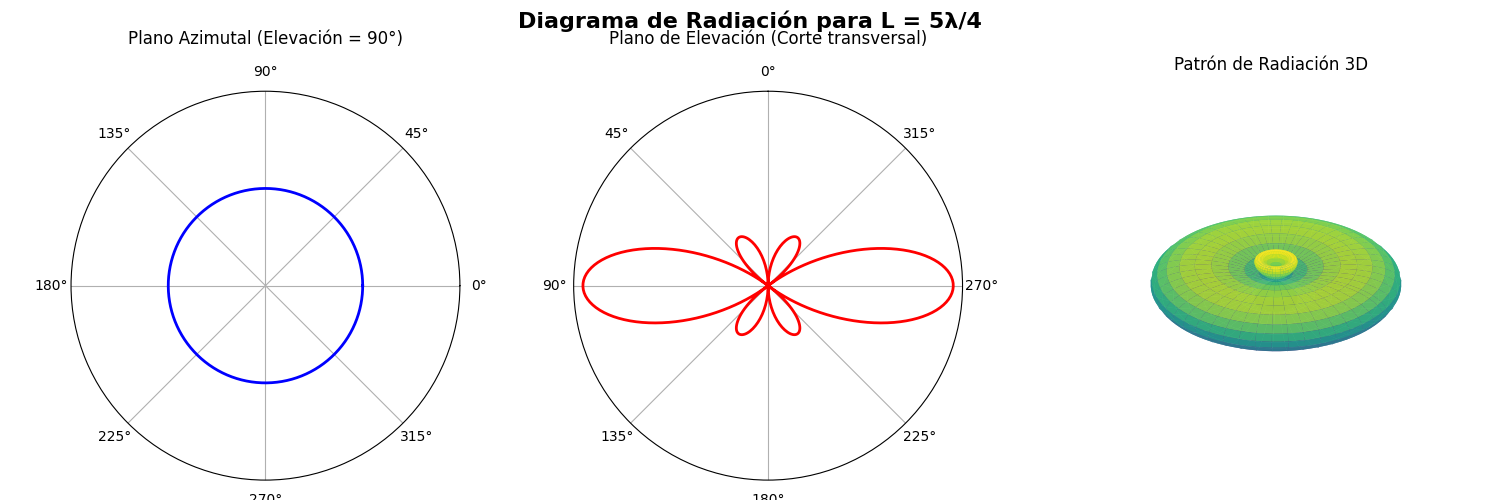
\includegraphics[width=1\linewidth]{Figura 7.png}
        \caption{Diagrama de Radiación para $L = \frac{5\lambda}{4}$.}
        \label{fig:fig_7}
    \end{figure}

    \item \underline{Diagrama de Radiación para $L = \frac{3\lambda}{2}$:}
    \begin{figure}[H]
        \centering
        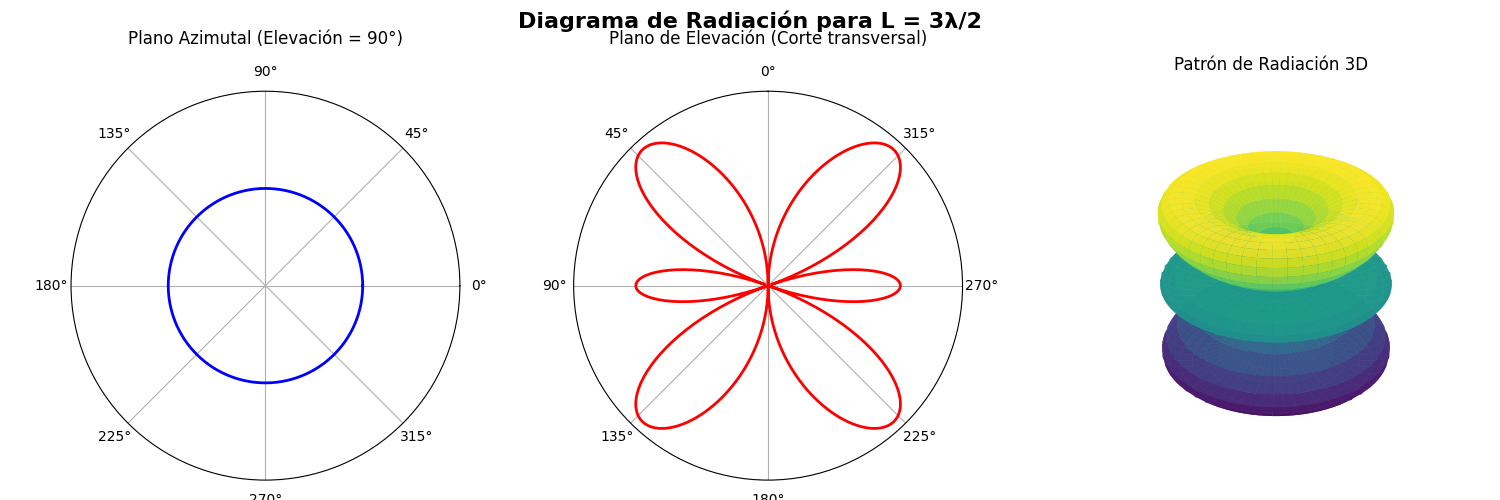
\includegraphics[width=1\linewidth]{Figura 8.png}
        \caption{Diagrama de Radiación para $L = \frac{3\lambda}{2}$.}
        \label{fig:fig_8}
    \end{figure}

    \item \underline{Diagrama de Radiación para $L = \frac{7\lambda}{4}$:}
    \begin{figure}[H]
        \centering
        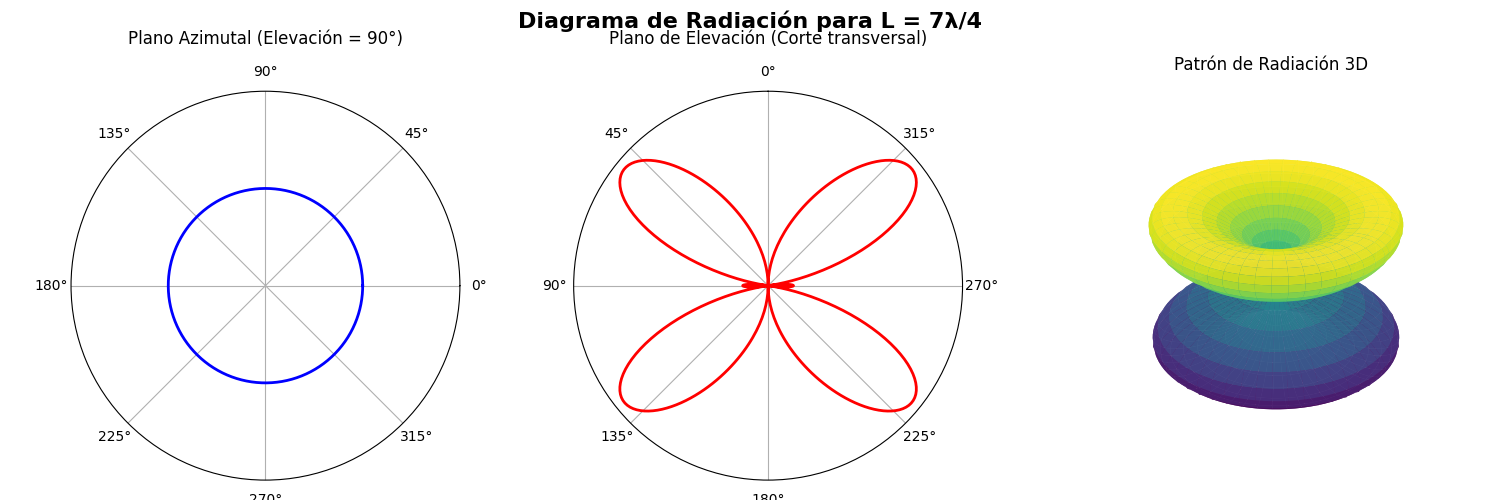
\includegraphics[width=1\linewidth]{Figura 9.png}
        \caption{Diagrama de Radiación para $L = \frac{7\lambda}{4}$.}
        \label{fig:fig_9}
    \end{figure}

    \item \underline{Diagrama de Radiación para $L = 2\lambda$:}
    \begin{figure}[H]
        \centering
        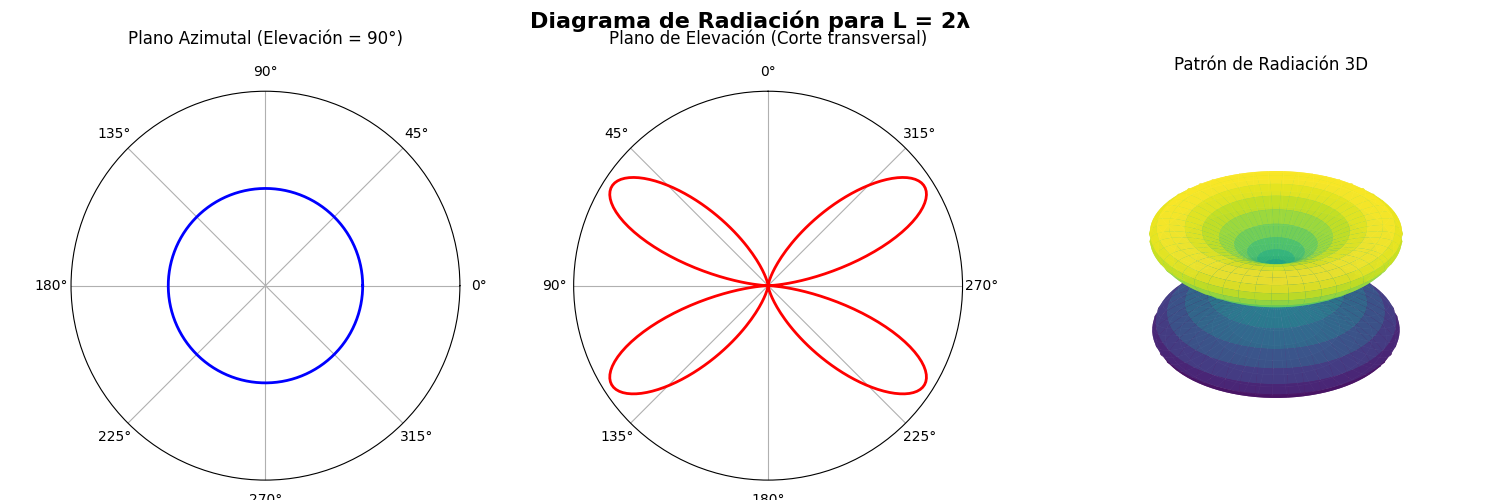
\includegraphics[width=1\linewidth]{Figura 10.png}
        \caption{Diagrama de Radiación para $L = 2\lambda$.}
        \label{fig:fig_10}
    \end{figure}

    \item \underline{Diagrama de Radiación para $L = \frac{9\lambda}{4}$:}
    \begin{figure}[H]
        \centering
        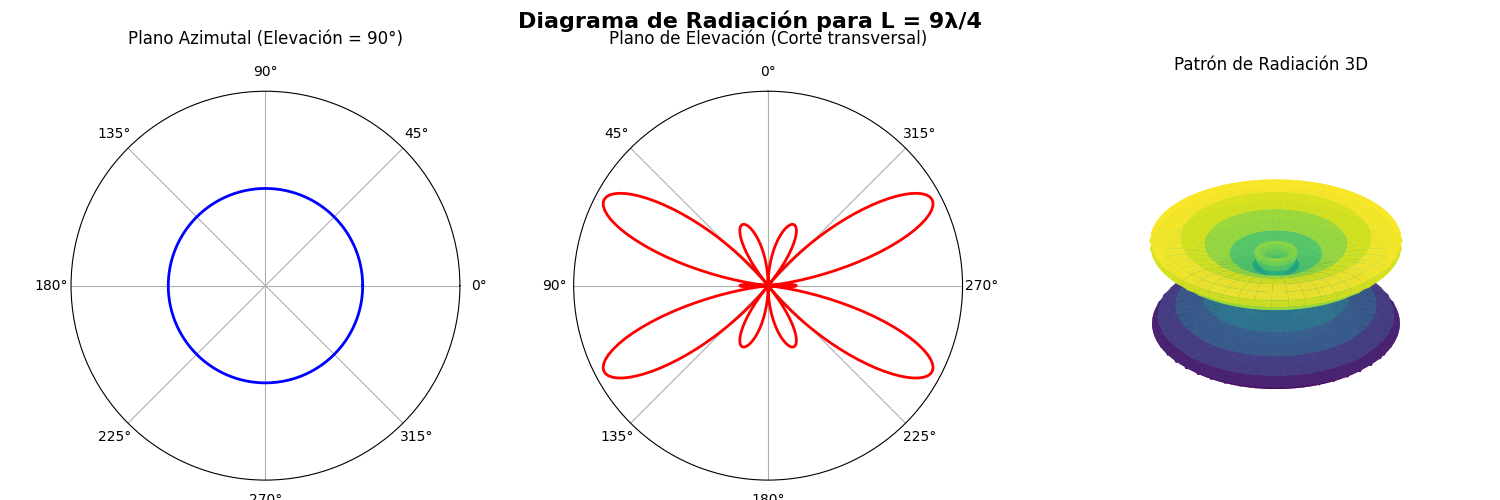
\includegraphics[width=1\linewidth]{Figura 11.png}
        \caption{Diagrama de Radiación para $L = \frac{9\lambda}{4}$.}
        \label{fig:fig_11}
    \end{figure}
\end{itemize}



\section{Conclusiones}
De acuerdo a las gráficas obtenidas en la sección precedente, se pueden realizar las siguientes conclusiones de acuerdo a los dipolos:
\begin{itemize}
    \item \underline{Dipolos Cortos e Intermedios ($L \le \lambda$):} Para longitudes físicas pequeñas en relación con la longitud de onda, como $\lambda/8$ y $\lambda/4$, el patrón de radiación mantiene una geometría puramente toroidal (en forma de "dona") y simétrica, siendo prácticamente idéntico al de un dipolo infinitesimal. Al alcanzar el clásico dipolo de media onda ($L = \lambda/2$), el haz en el plano de elevación se estrecha levemente, concentrando mayor energía y presentando su máxima radiación en la dirección perpendicular al eje de la antena ($\theta = 90^\circ$).Si se continúa incrementando la longitud hacia $3\lambda/4$ y hasta llegar al dipolo de onda completa ($L = \lambda$), el lóbulo principal no se divide ni se anula; por el contrario, experimenta un estrechamiento progresivo en el plano ecuatorial ($\theta = 90^\circ$). En $L = \lambda$, la directividad en dicha dirección alcanza su punto óptimo para un único lóbulo, debido a que la distribución de corriente a lo largo de todo el conductor se mantiene en fase, maximizando la interferencia constructiva en el plano horizontal.

    \item \underline{Dipolos Largos ($L > \lambda$):} Una vez que la longitud total del dipolo supera la longitud de onda de operación, el comportamiento del patrón cambia drásticamente debido a la naturaleza estacionaria de las ondas de corriente. Al ser el conductor lo suficientemente largo, la corriente comienza a sufrir inversiones de fase en distintas secciones del dipolo. A partir de $L = 5\lambda/4$, esta alternancia de fases provoca que los campos electromagnéticos radiados dejen de sumarse constructivamente en su totalidad, dando origen a los primeros lóbulos secundarios de carácter oblicuo. En el caso de $L = 3\lambda/2$, la radiación directa a $90^\circ$ disminuye de forma notoria, y la mayor parte de la potencia se desplaza hacia los lóbulos oblicuos, fragmentando el corte bidimensional en 6 lóbulos bien definidos.Finalmente, al alcanzar el dipolo de doble onda ($L = 2\lambda$), la cancelación de campos en la dirección perpendicular ($\theta = 90 \ [\degree]$) se vuelve absoluta. Esto genera un nulo de radiación perfecto en el centro debido a la interferencia destructiva simétrica entre las secciones de corriente que viajan en contra-fase. Como resultado, la energía se redistribuye por completo en el espacio, dividiendo el diagrama de radiación en un patrón complejo de 8 lóbulos perfectamente definidos e inclinados respecto al eje de la antena. [2]
\end{itemize}



\section{Bibliografía}
\begin{itemize}
    \raggedright
    \item \underline{$[1]$:} Calculisto. (s.f.). \textit{Cónicas y cuádricas: Resumen del tema} [Plataforma educativa]. \url{https://www.calculisto.com/topics/conicas-y-cuadricas/summary/824}

    \item \underline{$[2]$:} Johnk, C. T. A. (1988). Radiation from antennas in free space (Cap. 11). En \textit{Engineering Electromagnetic Fields and Waves} (2.ª ed.). John Wiley \& Sons. Recuperado de \url{http://linux0.unsl.edu.ar/~froma/libros/Jhonk2.pdf}

    \item \underline{$[3]$:} Monja, E. (s.f.). \textit{Diagramas de Radiación en Python.py} (Versión principal) [Código de software]. GitHub. \url{https://github.com/ErnestMonja/Antenas-y-Propagacion-de-Ondas/blob/main/Trabajo%20Pr%C3%A1ctico%20N%C2%B01%20-%20Diagrama%20de%20Radiaci%C3%B3n%20de%20la%20Antena%20Dipolo/Diagramas%20de%20Radiaci%C3%B3n%20en%20Python.py}
\end{itemize}
\end{document}
